\documentclass[a4paper]{article}

\usepackage[english]{babel}
\usepackage[utf8]{inputenc}
\usepackage[framed,numbered,autolinebreaks,useliterate]{mcode}
\usepackage{amsmath}
\usepackage{amssymb}
\usepackage{caption}
\usepackage{subcaption}
\usepackage[]{algorithm2e}
\usepackage[noend]{algpseudocode}
\usepackage{graphicx}
\usepackage{qtree}
\usepackage[colorinlistoftodos]{todonotes}

\makeatletter
\def\BState{\State\hskip-\ALG@thistlm}
\makeatother

\title{Project 4 Homomorphic filter}

\author{Johan Bowald and Anton Johansson}

\date{\today}

\begin{document}

\maketitle

\newpage

\section{Introduction}

The goal of the project is to visually enhance an black and white image of a forest scenery using Homomorphic Filtering(from here referred to as \textit{HF}). \\

This report present the design of a HF that the project group finds visually pleasing. 
The method of application is the same as described in the course book in chapter 4.9.6 Homomorphic Filtering but using the highpass gaussian filter described in 4.9.3 Gaussian Highpass Filters \cite{dipBook}. \\

A parameter study of the filters parameters and theirs contribution to the enhanced image followed up by the recommended parameters the group found most visually pleasing. Finally, the conclusion of either the technique is recommended for this type image and application. This conclusion is based on using the same technique on other types of images.
\section{Method}

An image $f(u,v)$ can be represented using an illumination-reflectance model. 
\begin{figure}[h!]
\begin{equation}
  f(u,v) = i(u,v) r(u,v)
  \label{eqn:im1}
\end{equation}
\caption{Image $f$ represented with an illumination component $i$ and reflection component $r$}
\end{figure}
The illumination $i(u,v)$ can be characterized as slow changes in the frequency domain or as glooming light in the spatial domain. While the reflection $r(u,v)$ tends to be rapid changes in the frequency domain or as edges in the spatial domain. The homomorphic filter works in the frequency domain and aims to filter out major influences of the illumination $i(u,v)$. This results in a higher contrast and normalized brightness. \\

\subsection{Pre-pocessing of the original image}
To apply the filter the image $f(u,v)$ needs to be transformed into frequency domain. Since the illumination-reflectance model is multiplicative and will result in a convolution in frequency space the image will need to be pre-processed before the transformation.

\begin{figure}[h!]
\begin{equation}
  \mathfrak{F}[f(u,v)] = \mathfrak{F}[i(u,v)] \ast \mathfrak{F}[r(u,v)] 
  \label{eqn:transWithoutLogRes}
\end{equation}
\begin{equation}
  \mathfrak{F}[f(u,v)] \neq \mathfrak{F}[i(u,v)] \mathfrak{F}[r(u,v)] 
  \label{eqn:transWithoutLogErr}
\end{equation}
\caption{Multiplication will become convolution (\ref{eqn:transWithoutLogRes}) in frequency domain and not remain multiplicative.(\ref{eqn:transWithoutLogErr})}
\end{figure}

Applying the logarithmic transformation on the original image results in a transformation of the illumination-reflectance model from multiplicative to additive, Eq \ref{eqn:loga}. The Fourier transform is applied to the resulting image of the logarithmic transform and the illumination-reflectance model is intact and in frequency domain as seen in EQ \ref{eqn:logtrans}
\begin{figure}[h!]
\begin{equation}
  f(u,v) = i(u,v) r(u,v) \xrightarrow{\ln} \ln{f(u,v)} = \ln{i(u,v)} + \ln{r(u,v)} 
  \label{eqn:loga}
\end{equation}
  \begin{equation}
    \begin{split}
      Z(u,v) &= \mathfrak{F} [\ln{f(u,v)}]\\ &= \mathfrak{F}[\ln{i(u,v)}] + \mathfrak{F}[\ln{r(u,v)}]\\ &= F_i(u,v) + F_r(u,v)
    \end{split}
    \label{eqn:logtrans}
  \end{equation}
\caption{image $f$ represented with an illumination component $i$ and reflection component $r$, in Eq \ref{eqn:loga} multiplication becomes additive after logarithmic transform. Eq \ref{eqn:logtrans} shows the result of a fourier and logarithmic transformed image $Z$ and the corresponding illumination and reflection component.}
\end{figure}

Since the images are discrete and the Fourier Transform is applied to infinity, matlab will loop the input image periodically. To avoid aliasing and introduction of errors when applying the filter to the image, the input image is zero padded. Zero Padding the source image using matlabs \verb~padarray~ -function. The amount of zeros padded with the image is calculated using equations \ref{eqn:Ppadded} and \ref{eqn:Qpadded} given in the coursebook\cite[p. 274]{dipBook}. Exempel of zero padding is shown in Figure \ref{fig:zeropadded}.
\begin{figure}[h!]
\begin{equation}
  P \geq 2M -1
  \label{eqn:Ppadded}
\end{equation}
\caption{4.6-31, P: Resulting vertical size of the image, M: vertical size of source image}
\end{figure}

\begin{figure}[h!]
  \begin{equation}
    Q \geq 2N -1
    \label{eqn:Qpadded}
  \end{equation}
  \caption{4.6-31, Q: Resulting horisontal size of the image, N: horizontal size of source image}
\end{figure}

\begin{figure}[h!]
  \begin{center}
    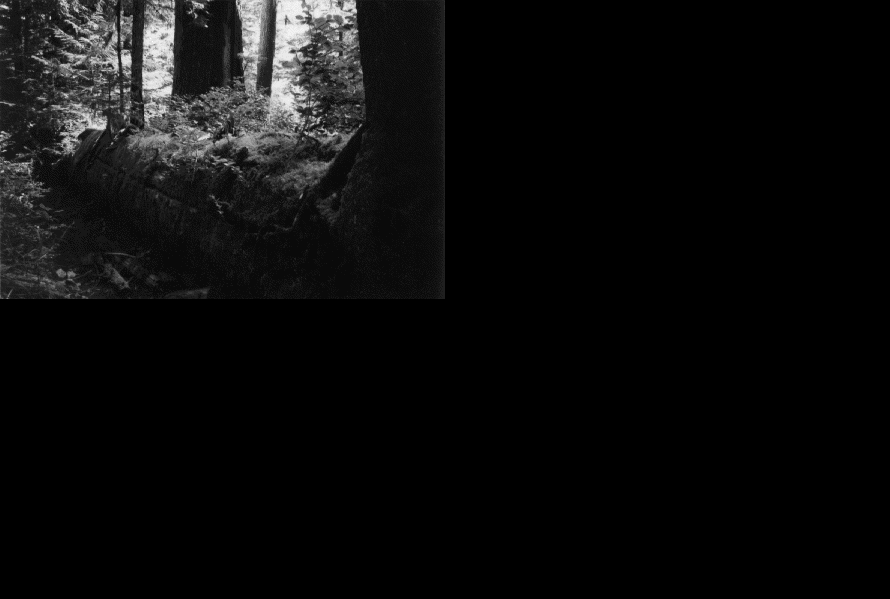
\includegraphics[width=0.6\textwidth]{pics/zeroPadded.png}
  \end{center}
  \cprotect\caption{Original image padded with P-M and Q-N zeros after original matrix using \verb~padarray~ in matlab.}
  \label{fig:zeropadded}    
\end{figure}

The filter used in this project is center positioned. Since matlabs \verb~fft2~ returns the transformed image with the origio in upper left corner, the result must be shifted to apply the filter correctly. Shifting the transformation is done using matlabs \verb~fftshift~

\subsection{The construction of the homomorphic filter}
The filter used to enhanced the image in this project is a highpass gaussian filter,Eq \ref{eqn:gaussian_filter}, with three parameters. 
    \begin{equation}
    \label{eqn:gaussian_filter}
      H(u,v) = \left( \gamma_H - \gamma_L \right) \left[ 1 - e^{- D(u,v) /2 \cdot D_0^2}\right] + \gamma_L 
    \end{equation}

\begin{itemize}
  \item $\gamma_H$ sets the maximum amplitude of the filter.
  \item $\gamma_L$ sets the lower bound of amplitude of the filter.
  \item $D_0$ is the cut-of frequency, to control the steepness and width of the gaussian function.
  \item The function $D(u,v)$ calculates the distance from the center of the filter to each element ,$u,v$, in the filter.  
\end{itemize}

\begin{figure}[h!]
  \begin{lstlisting}
    [u, v] = meshgrid(1:q,1:p);
    centerU = ceil(q/2);
    centerV = ceil(p/2);
    gaussianNumerator = ((u - centerU).^2 + (v - centerV).^2);
  \end{lstlisting}
  \label{code:raduv}
  \caption{Matlab code of the distance function $D(u,v)$ used in the filter. p and q is the size of the image after zero padding.}
\end{figure}

\subsection{Applying the filter and the post-processing}

The filter is applied by multiplication in the Frequency domain as seen in Figure \ref{fig:filteringOfImage}. 
\begin{figure}[h!]
  \begin{equation}
    S(u,v) = Z(u,v)H(u,v)
    \label{eqn:applyfilt}
  \end{equation}
  \caption{S: the filtered image, Z: pre-processed image from Eq \ref{eqn:logtrans}, H: highpass guassian filter described in Eq \ref{eqn:gaussian_filter} }
  \label{fig:filteringOfImage}    
\end{figure}

Post-processing consists of four steps.

\begin{enumerate}
  \item Shifting the filtered image to get the origin in top/left corner.
  \item Apply the inverse fourier transform. Crop the zero padding to obtain the original image dimensions.
  \item Crop the zero padding to obtain the original image dimensions.
  \item Inverse logarithmic transformation by taking the exponential function of the result of cropped image.
\end{enumerate}

The result of the post-process is homomorphic filtered image. 
% \documentclass[a4paper]{article}
% \usepackage{graphicx}
% \usepackage{caption}
% \usepackage{subcaption}
% \begin{document}


\section{Results}
	This section will present the results of applying homomorphic filtering
	on an image. Also provided is some experiments with different images
	and filters not used in the book, as to test if this method could yield
	better or worse results in different types of information depicted.
	\subsection{Results on the image provided with the project}
		The image provided with the project depicts a forest scenery. %include picture
		As seen in figure [INSERT IMAGE HERE] it %Har väl inga direkta större
		% inslag av kraftig illumination
		
		The filter first used in this project was
		the gaussian high-pass filter detailed in the course book on pp. 314; 
		%
		\begin{equation}
		\label{eqn:gaussian_filter}
			H(u,v) = \left( \gamma_H - \gamma_L \right) \left[ 1 - e^{-c \left[D^2(u,v)/D_0^2\right]}\right] + \gamma_L 
		\end{equation}
		 %
		This filter has the additional $\gamma$-parameters added in order to tweak
		the filter in regard to illumination and reflection. The $\gamma_L$ parameter
		will define the amount of suppression of the low frequencies (illumination); a lower $\gamma_L$
		will suppress low frequencies, which can be seen in figure~\ref{fig:various_low_gamma}. While
		figure~\ref{fig:low_freq_supp} may not be the most pleasurable image to look at, but it 
		enhances the information hidden in the low frequencies, especially in the darker areas.
		\begin{figure}[h!]
		\centering
		\begin{subfigure}[b]{0.6\textwidth}
			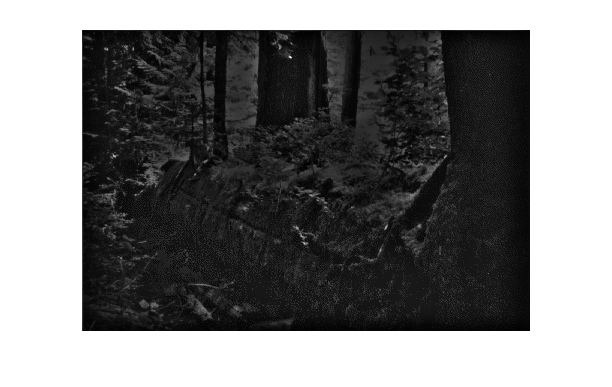
\includegraphics[width=\textwidth]{pics/suppressed_low_frequences.png}
			\caption{$\gamma_L = 0.01,~\gamma_H = 1$}
			\label{fig:low_freq_supp}
			\end{subfigure}%			
			\begin{subfigure}[b]{0.6\textwidth}
			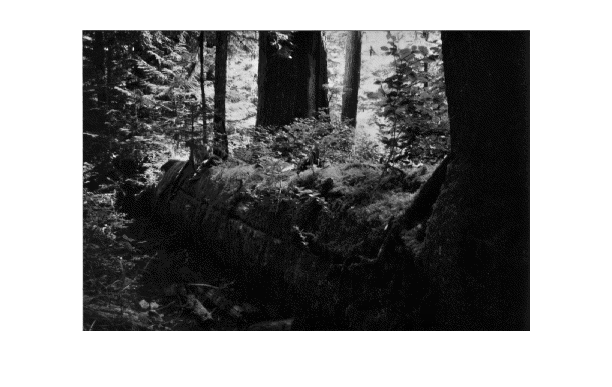
\includegraphics[width=\textwidth]{pics/non_suppressed_low_frequences.png}
			\caption{$\gamma_L = 0.8,~\gamma_H = 1$}
			\label{fig:low_freq_non_supp}
			\end{subfigure}
			\label{fig:various_low_gamma}
			\caption{The effect of changing $\gamma_L$}				
		\end{figure}		
		%
		A large value of the $\gamma_H$ parameter 
		will emphasize the high frequencies (reflection). As an example, 
		examine figure~\ref{fig:gamma_diff}.
		\begin{figure}[h!]
			\centering
			\begin{subfigure}[b]{0.6\textwidth}
				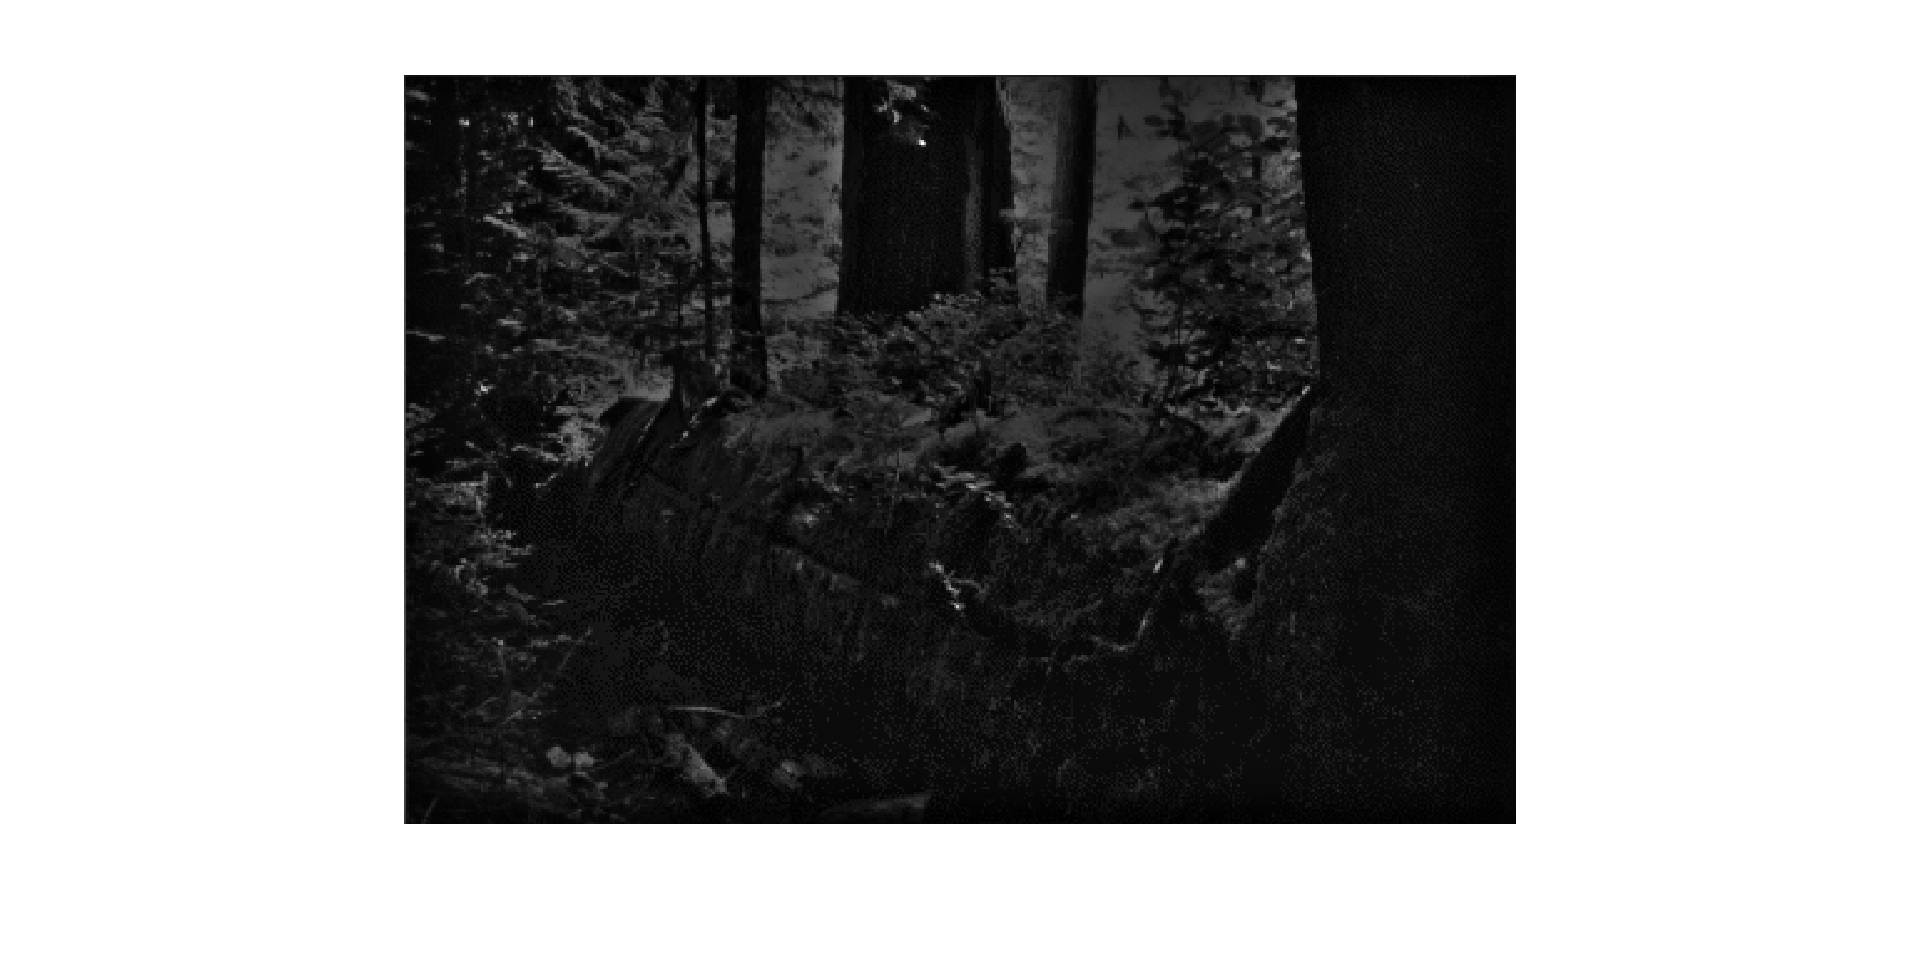
\includegraphics[width=\textwidth]{pics/non_emph_high_frequnces.png}
				\caption{$\gamma_L = 0.3,~\gamma_H = 1.2$}
				\label{fig:high_freq_non_emph}
			\end{subfigure}%	
			\begin{subfigure}[b]{0.6\textwidth}
				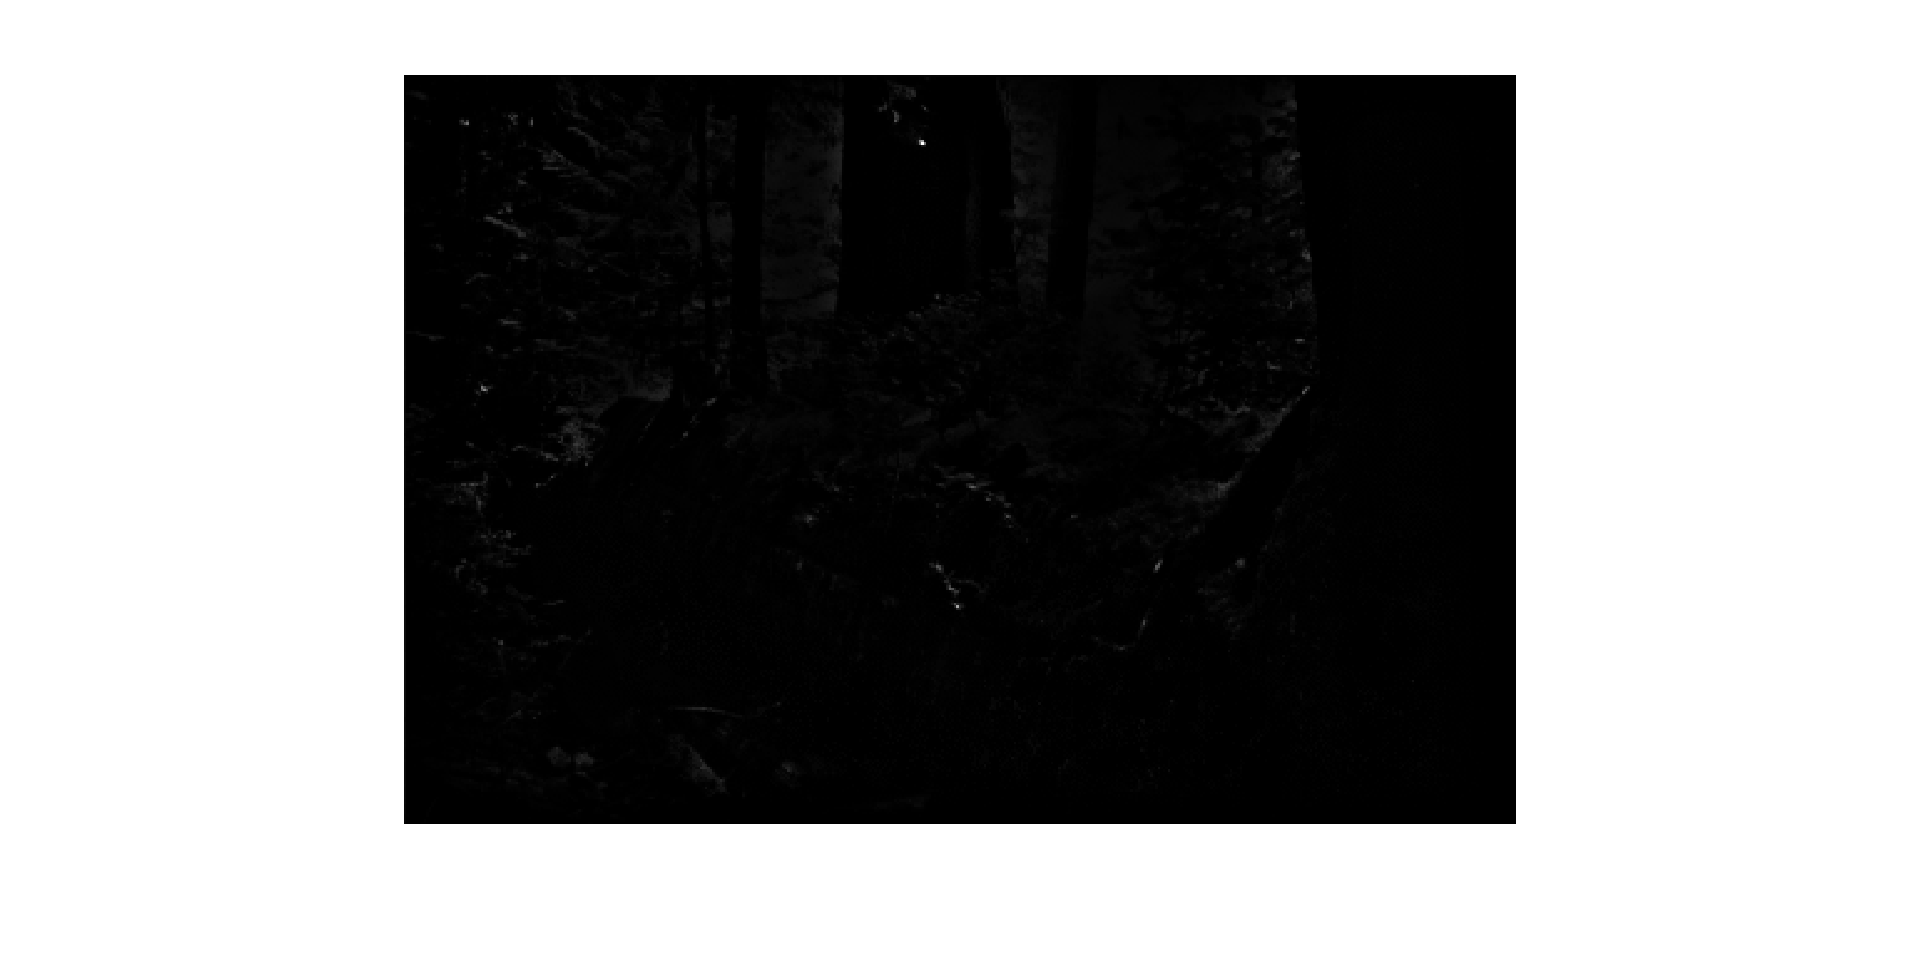
\includegraphics[width=\textwidth]{pics/emph_high_frequnces.png}
				\caption{$\gamma_L = 0.3,~\gamma_H = 2.5$}
				\label{fig:high_freq_emph}
			\end{subfigure}
			\label{fig:high_gamma}
		\caption{The effect of changing $\gamma_H$}				
		\end{figure}		
		One is able to see that the reflections gets emphasized and the overall
		image gets darker and more polarized.
		The third and final parameter is $D_0$, which controls the steepness of the filter.
		In practice, this means that a larger $D_0$ will produce an image with a more 
		narrow spectra of gray levels. The effect of this is visible in figure~\ref{fig:sigma}
		\begin{figure}[h!]
			\centering
			\begin{subfigure}[b]{0.7\textwidth}
				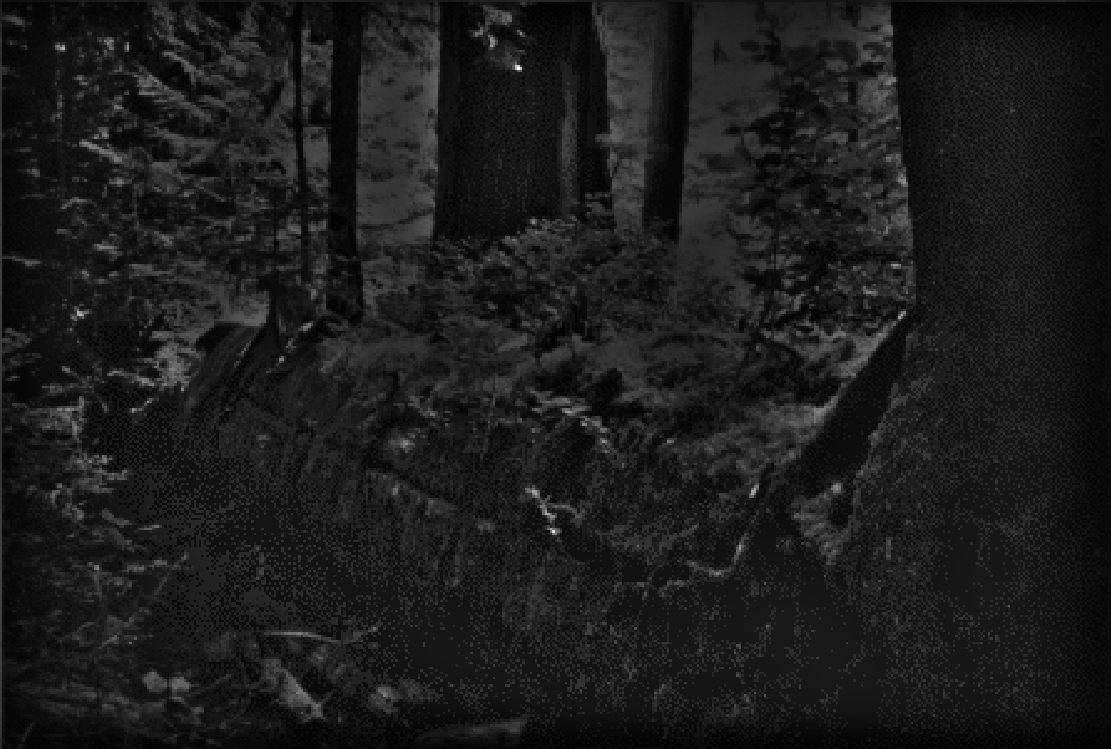
\includegraphics[width=\textwidth]{pics/low_sigma.png}
				\caption{$\gamma_L = 0,~\gamma_H = 1,~D_0 = 10$}
				\label{fig:low_sigma}
			\end{subfigure}%
			\begin{subfigure}[b]{0.7\textwidth}
				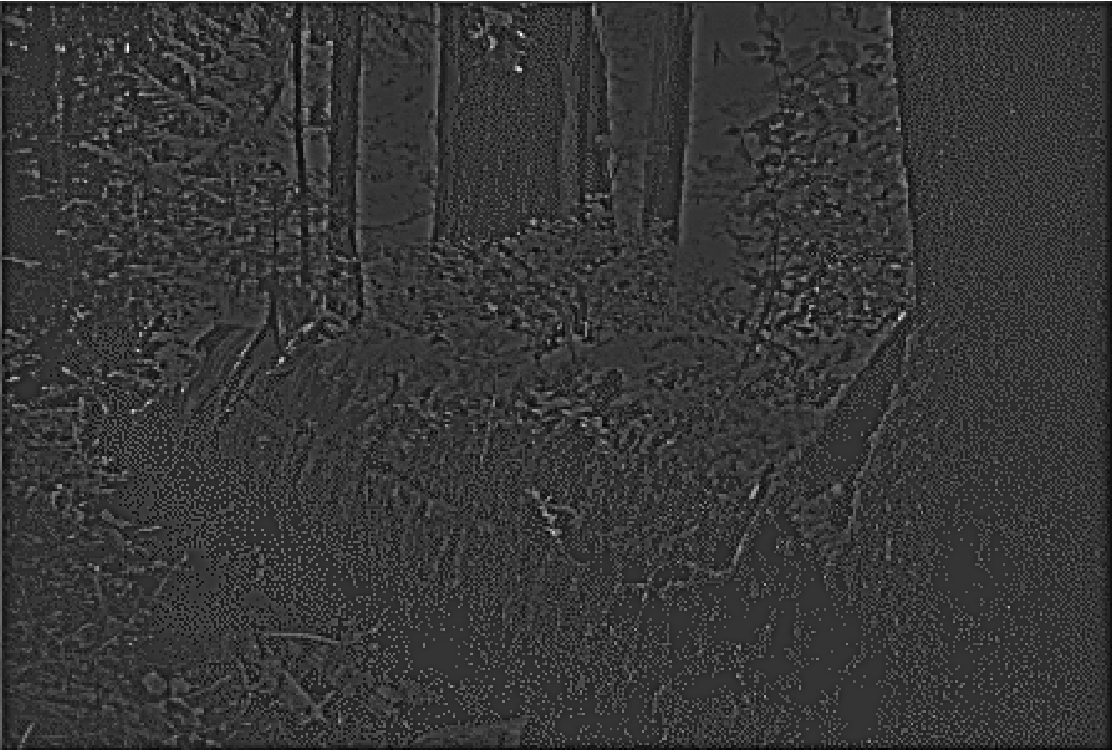
\includegraphics[width=\textwidth]{pics/high_sigma.png}
				\caption{$\gamma_L = 0,~\gamma_H = 1,~D_0 =80$}
				\label{fig:high_sigma}
			\end{subfigure}
			\label{fig:sigma}
			\begin{subfigure}[b]{0.6\textwidth}
				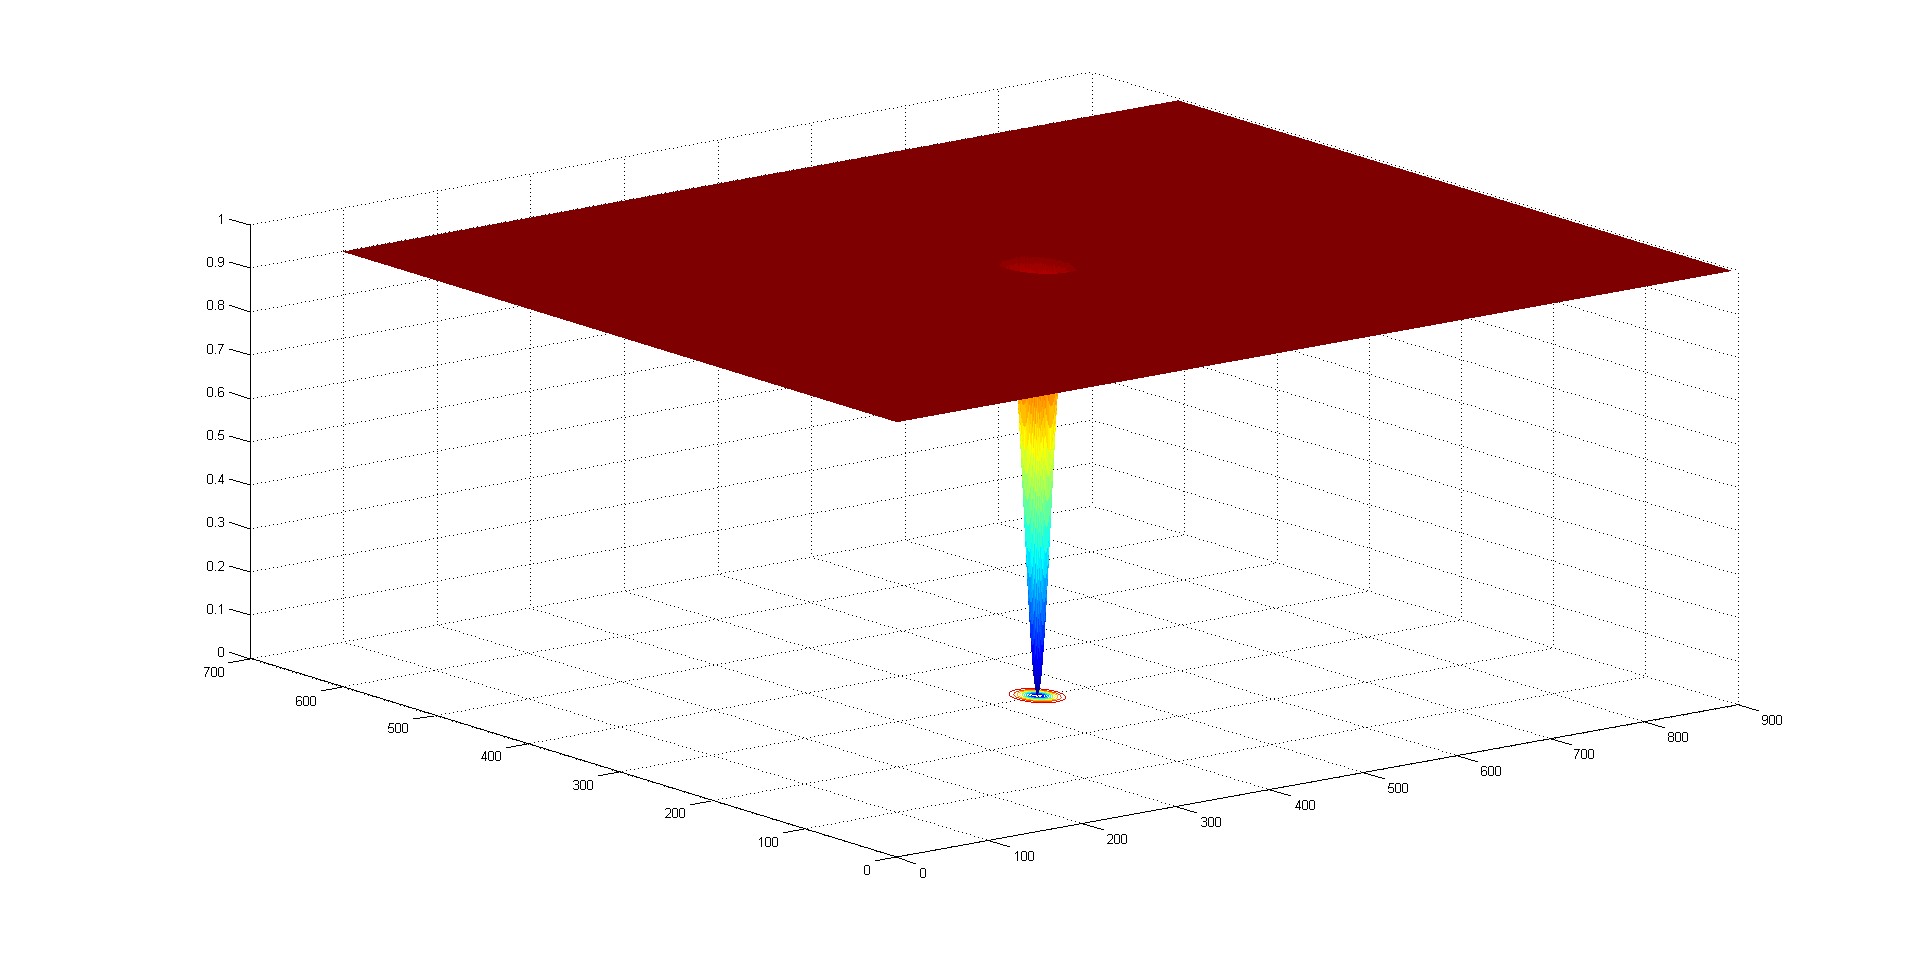
\includegraphics[width=\textwidth]{pics/low_sigma_filter.png}
				\caption{}
				\label{fig:low_sigma_filter}
			\end{subfigure}%
			\begin{subfigure}[b]{0.6\textwidth}
				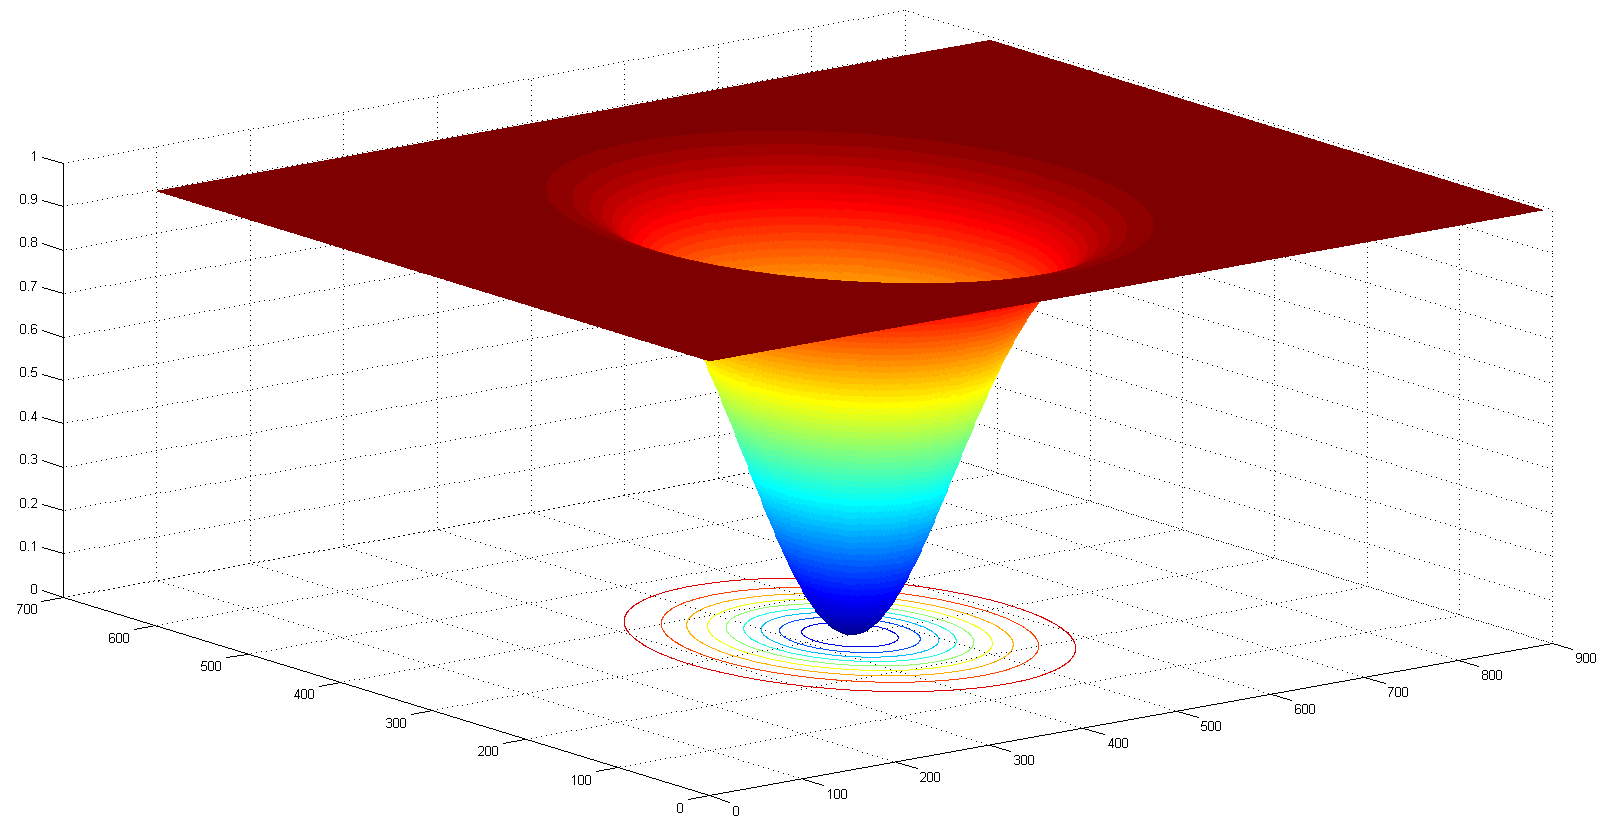
\includegraphics[width=\textwidth]{pics/high_sigma_filter.png}
				\caption{}
				\label{fig:high_sigma_filter}
			\end{subfigure}
			\label{fig:sigma}
		\caption{The effect of changing $D_0$, with the corresponding filter below each result}				
		\end{figure}
		with the corresponding filters. A very high $D_0$ is moving close to edge detection,
		which can be very useful in areas such as computer vision, which is described in 
		the paper \emph{Homomorphic filtering based illumination normalization 
		method for face recognition} by Fan, Zhang.
		\\
		Various $\gamma_l$ and $\gamma_h$ paramaters has been tried out empirically with 
		various results. One has to ask oneself; What information should be extracted, and what 
		method performs best? When experimenting with emphasizing the reflections, the 
		general results was not very good. Usually the image got very dark with a few white
		spots from the highest frequencies, like in figure~\ref{fig:high_freq_emph}.
		\\
		When observing the original image, there seems to be some 
		low frequency details hidden in the darker sections of the image which we were able
		to enhance. When the paramaters was $\gamma_L = 0,~\gamma_H = 1$,
		essentially elimiting the use of the parameters, a (in our opinion) good result was 
		found in figure~\ref{fig:result}. The details in the darker sections gets enhanced, 
		and the overall brightness
		of the image gets equalized. One drawback is that the bushes, which details 
		and structure seems consist
		largely of illumination, gets suppressed and blends in with the background.\\
		Further the other parameters was set to $c = 0$ and $D_0 = 32$. Of course,
		the paramaters should be changed depending on what information should be extracted.
		Our final conclusion when working on this image is that homomorphic filtering
		is probably not the best method to use in order to enhance it.
		\begin{figure}[h!]
			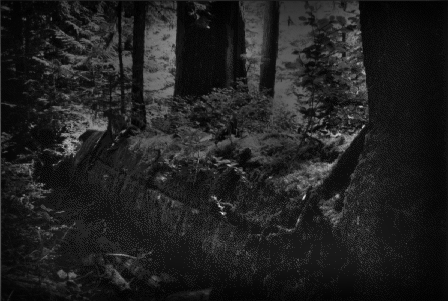
\includegraphics{pics/resulting_image.png}
			\caption{The result}
			\label{fig:result}		
		\end{figure}
							    
		\subsection{Experiments with different images}
		If homomorphic filtering is applied on images with a more appearent
		illumination distortion, such as figure~\ref{fig:gamma_diff} taken
		\begin{figure}[h!]
        \centering
% <<<<<<< HEAD
        % \begin{subfigure}[b]{0.6\textwidth}
        %         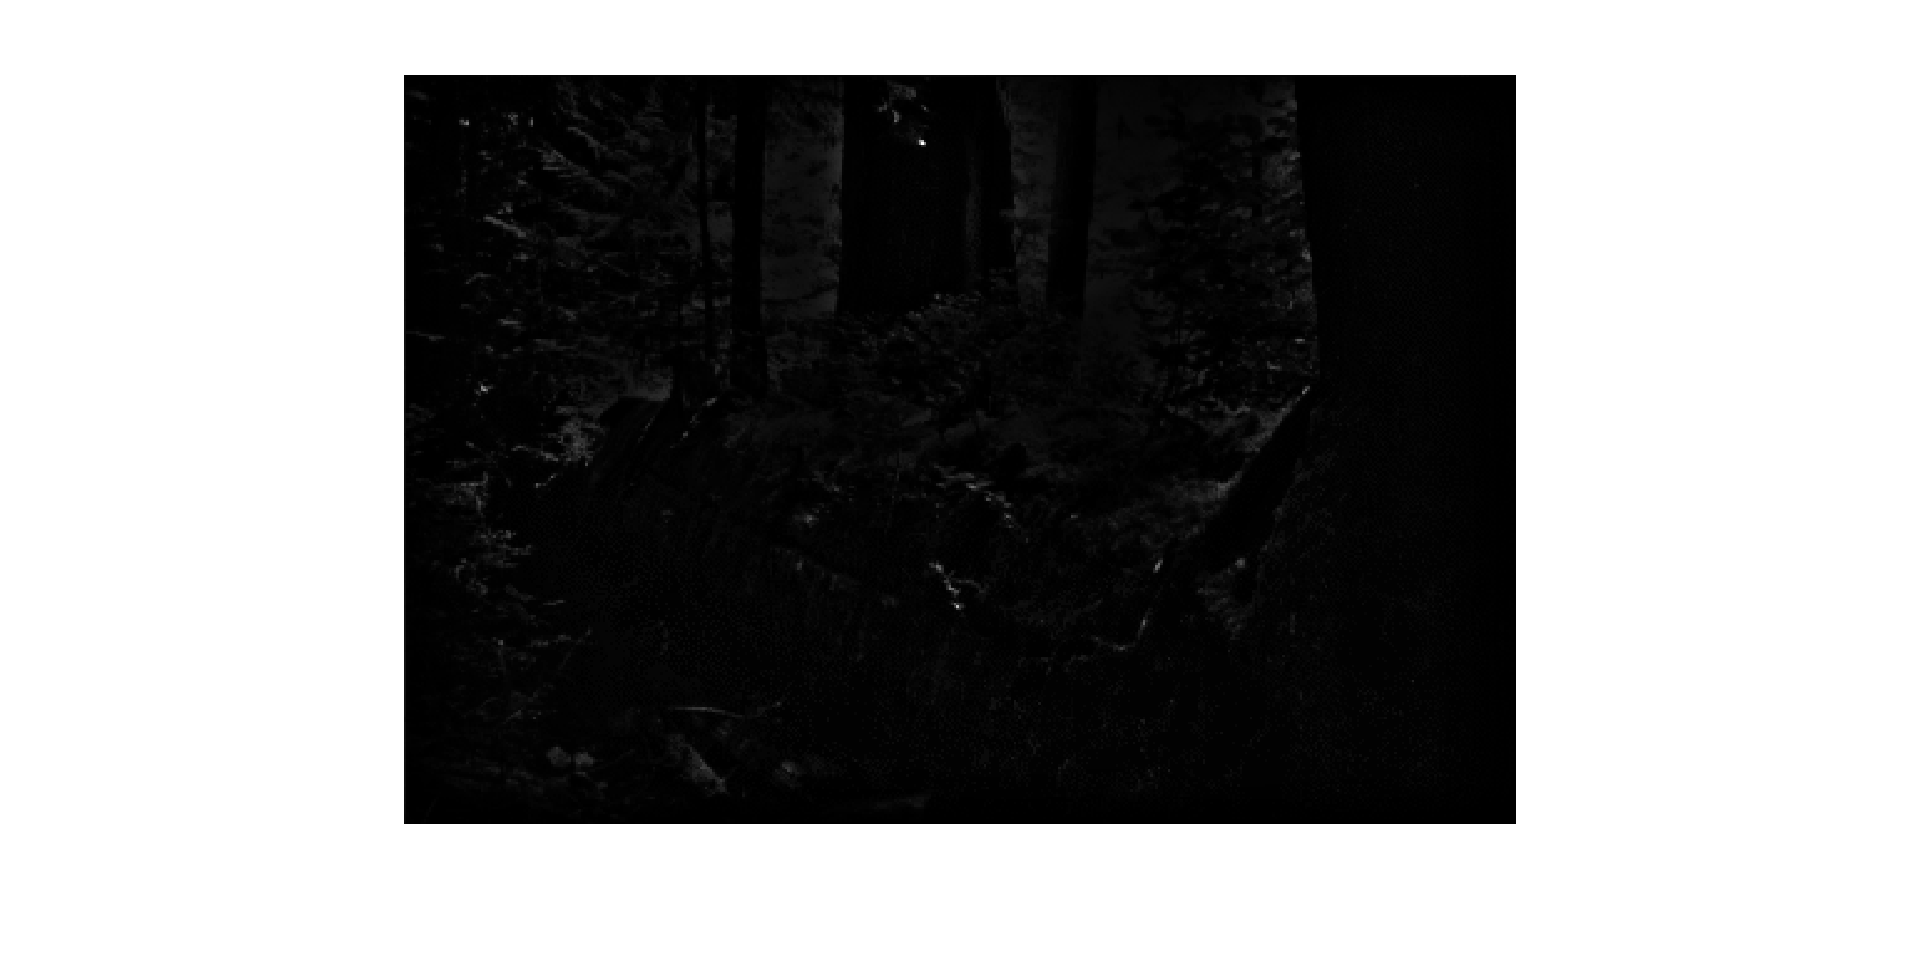
\includegraphics[width=\textwidth]{pics/gamma_difference_emph_lowfreq.png}
        %         \caption{$\gamma_L = 0.1,~\gamma_H = 2$}
        %         \label{fig:gamma_l_emph}
        % \end{subfigure}%
        % \begin{subfigure}[b]{0.6\textwidth}
        %         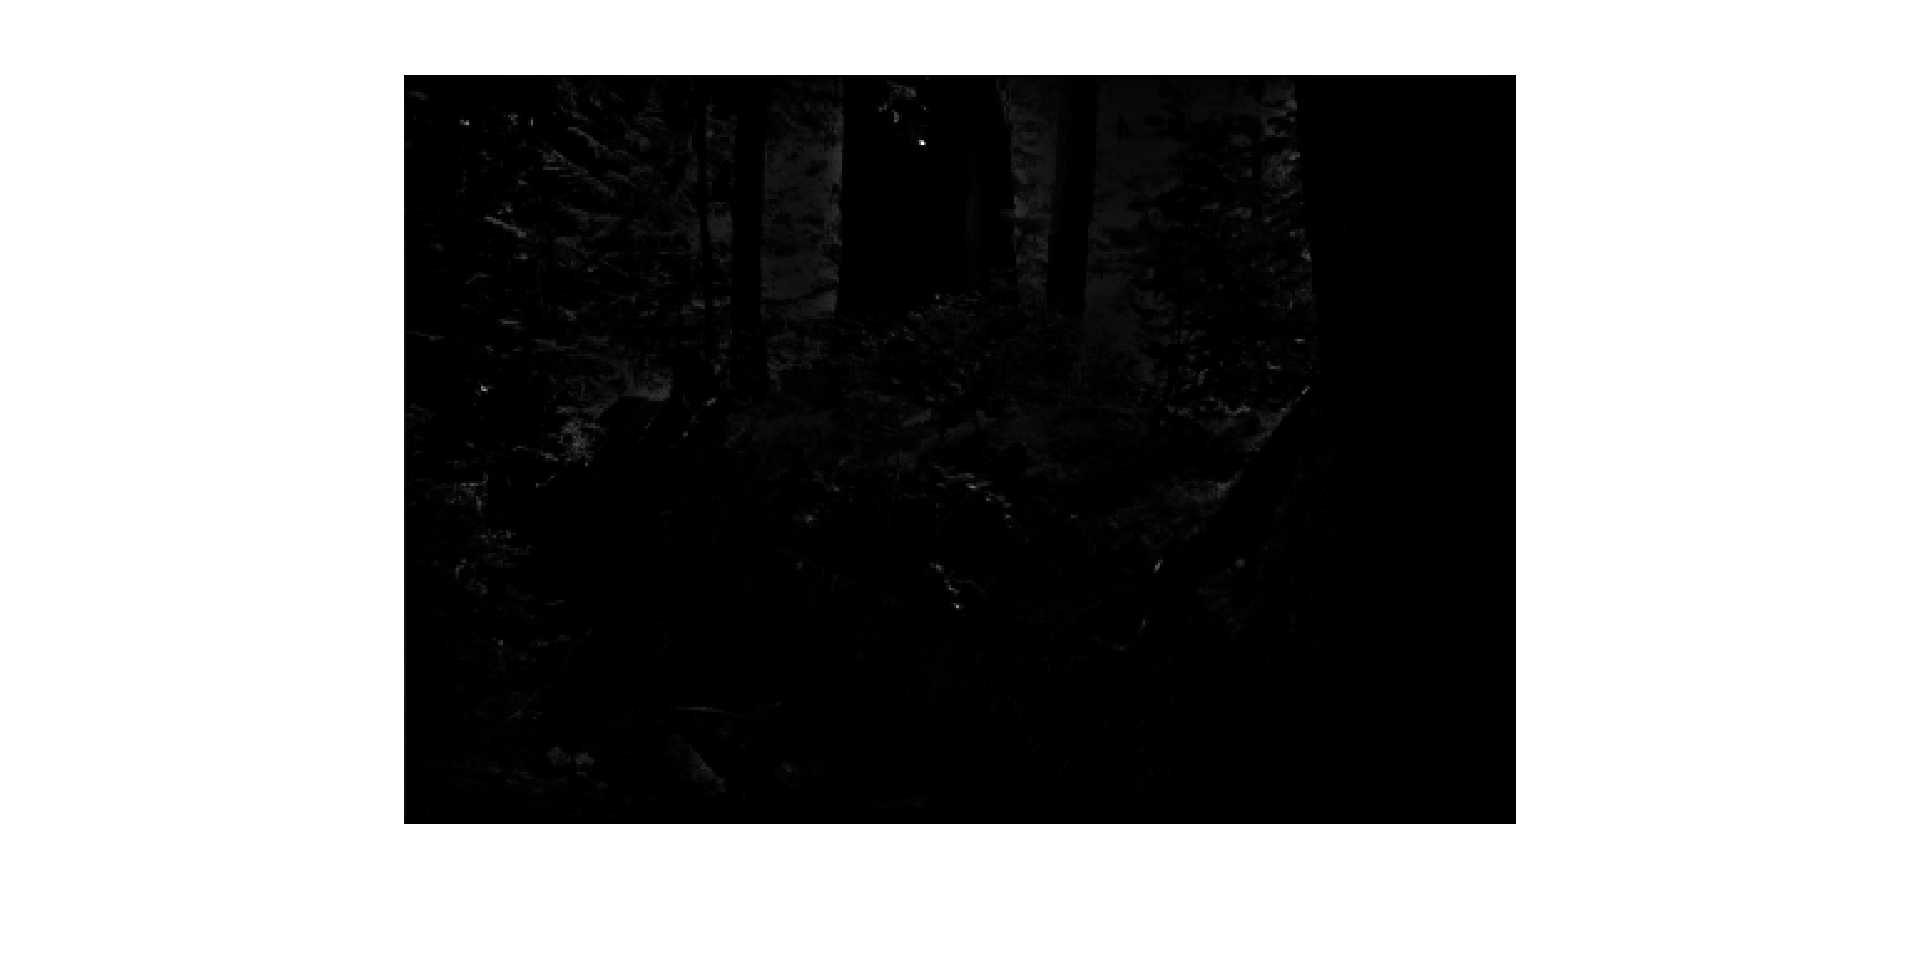
\includegraphics[width=\textwidth]{pics/gamma_difference_no_emph_lowfreq.png}
        %         \caption{$\gamma_L = 0.9,~\gamma_H = 2.8$}
        %         \label{fig:gamma_l}
% =======
		\begin{subfigure}[b]{0.6\textwidth}
                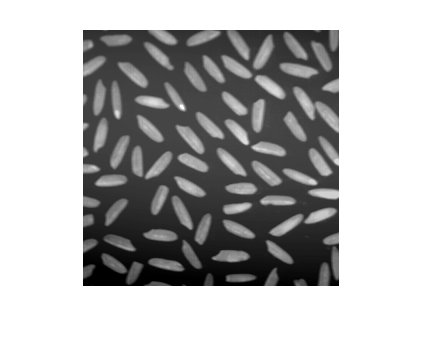
\includegraphics[width=\textwidth]{pics/microbes_before.png}
                \caption{Original image}
                \label{fig:microbe_before}
        \end{subfigure}%
        \begin{subfigure}[b]{0.6\textwidth}
                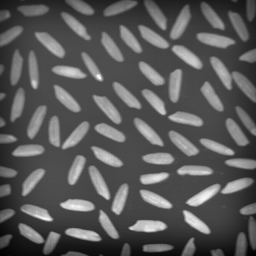
\includegraphics[width=\textwidth]{pics/microbes_after.png}
                \caption{Image after homomorphic filtering}
                \label{fig:microbe_after}
% >>>>>>> 89710fbfa1d52b28cbaa20bff4bb526a16a2c6f7
        \end{subfigure}
        \caption{An image with a appearent illumination distortion in the background}	
        \label{fig:gamma_diff}
		\end{figure}
		from the matlab image processing toolbox, the effects are much more obvious. 
		In this image there is a large illumination
		distortion in the background (the black gradient), which here is efficiently 
		removed by the homomorphic filtering process. \\
		\\
		When reading various papers on the
		subject we found several other areas where homomorphic filtering is very effective,
		such as a preprocessing step for facial recognition. The human face has many convex
		portions, which contributes to illumination. In the paper mentioned earlier, HF
		is used to remove this illumination and bring forth the edges in the face, making
		the facial recognition algorithms perform better under varying lightning conditions.
		%Elaborate perhaps?
% \end{document} 

\section{Discussion}

\end{document} 